%\chapter[Name in the PDF menu]{Name in the text (and index)}
\chapter{Experimental setup}
This thesis uses data obtained through the CMS experiment, which is one of the four major experiments operating at the CERN Large Hadron Collider (LHC).
CERN, the European Organisation for Nuclear Research, was founded in 1954 by a consortium of 12 European countries and its original programme was the study of atomic nuclei.
Over time, CERN's scientific endeavours have extended in parallel with the understanding of matter, and its current main research area is particle physics: the fundamental constituents and the forces that govern them.
To investigate fundamental interactions, particles are accelerated through a chain of of particle accelerators culminating (at the present day) with the LHC.
The collision products are observed and recorded by particle detectors, such as the CMS experiment.

\section{The Large Hadron Collider}
The Large Hadron Collider (LHC) \cite{CERN-AC-93-03-LHC}, situated at the European Organisation for Nuclear Research (CERN) in Geneva, is a massive, two-ring superconducting accelerator designed for high-energy particle collisions.
It operates within a circular underground tunnel spanning 26.7 kilometres, originally excavated to accommodate the LEP electron-positron collider, operating from 1989 to 2000.

The LHC accelerates two counter-rotating beams, primarily composed of protons but also capable of collision with heavy nuclei like lead (Pb) at varying energies.
The acceleration process involves a sequence of pre-accelerators, shown in Figure \ref{fig:CERNaccelerators}: the protons are isolated from a duoplasmatron source, accelerated through Linac2 to 50 MeV, further pushed in the Proton Syncrotron Booster (PSB) to 1.4 GeV, accelerated to 25 GeV in the Proton Synchrotron (PS), and finally reach an energy of 450 GeV in the Super Proton Synchrotron (SPS) before entering the LHC rings.
It was designed to accelerate protons up to 7 TeV ($\sqrt{s} =$ 14 TeV), and has successfully done so at 3.5 and 4 TeV during Run 1, at 6.5 TeV during Run 2 and 6.8 TeV during the ongoing Run 3.
Operation at 7 TeV is scheduled for the upcoming High Luminosity LHC (HL-LHC) after Long Shutdown 3.

\begin{figure}[htb]
\begin{center}
\includegraphics[width=0.85\textwidth]{pictures/CCC-v2017.png}
\end{center}
\caption{The CERN accelerator complex \cite{OPEN-PHO-ACCEL-2016-009}. The protons start from the LINAC2 and are accelerated by the Booster, the PS and SPS before reaching the LHC.}
\label{fig:CERNaccelerators}
\end{figure}

The LHC's design incorporates various types and sizes of magnets, each serving specific functions: dipole magnets bend the beams, quadrupole magnets focus the beams, and sextupole magnets compress the beams closer to the intersection points to increase the likelihood of particle interactions.
This highly sophisticated accelerator operates at temperatures as low as 1.9 K (-271.25 $^\circ$C) by utilising superfluid helium to cool and maintain the superconducting electromagnets capable of producing magnetic fields of 8.65 T.

Proton bunches in the LHC are spaced by 25 ns and cross at a rate of 40 MHz.
The nominal number of protons per bunch is $N_b = 12 \times 10^{11}$ and the nominal number of bunches is $2808$.

\section{The Compact Muon Solenoid experiment}
The Compact Muon Solenoid (CMS) is one of the two general purpose detectors operating at the LHC.
It is installed in a 100-meter deep cavern situated in the proximity of the French village of Cessy.
The detector was designed to cover a broad scope of physics analyses at the TeV scale, ranging from precision measurements of the electroweak observables to Beyond Standard Model (BSM) searches.
The main feature of the CMS experiment is its superconducting solenoid magnet with 6 m internal diameter and 12.5 m length, which provides a highly homogeneous magnetic field of 3.8 T.
The high field intensity allows the overall apparatus to be compact, compared to the other general purpose detector, ATLAS: it is 21.6 m long, 14.6 meter wide and weights 14000 tonnes.
The high bending power is needed to accurately measure the momentum of charged particles up to 1 TeV.
The fine granularity of the CMS detector over a large geometrical coverage allows achieving excellent muon identification and momentum resolution.
The other detector design goals are high resolution of the electromagnetic and hadronic energy deposition, as well as excellent tracking and vertexing.

In order to distinguish between particle signatures, and to provide the most precise measurements of their properties, CMS was built with an onion-like structure, each subdetector layer targeting a certain response.
A schematic diagram of CMS and its subdetectors is illustrated in Figure \ref{fig:CMSslice}.

\begin{figure}[htb]
\begin{center}
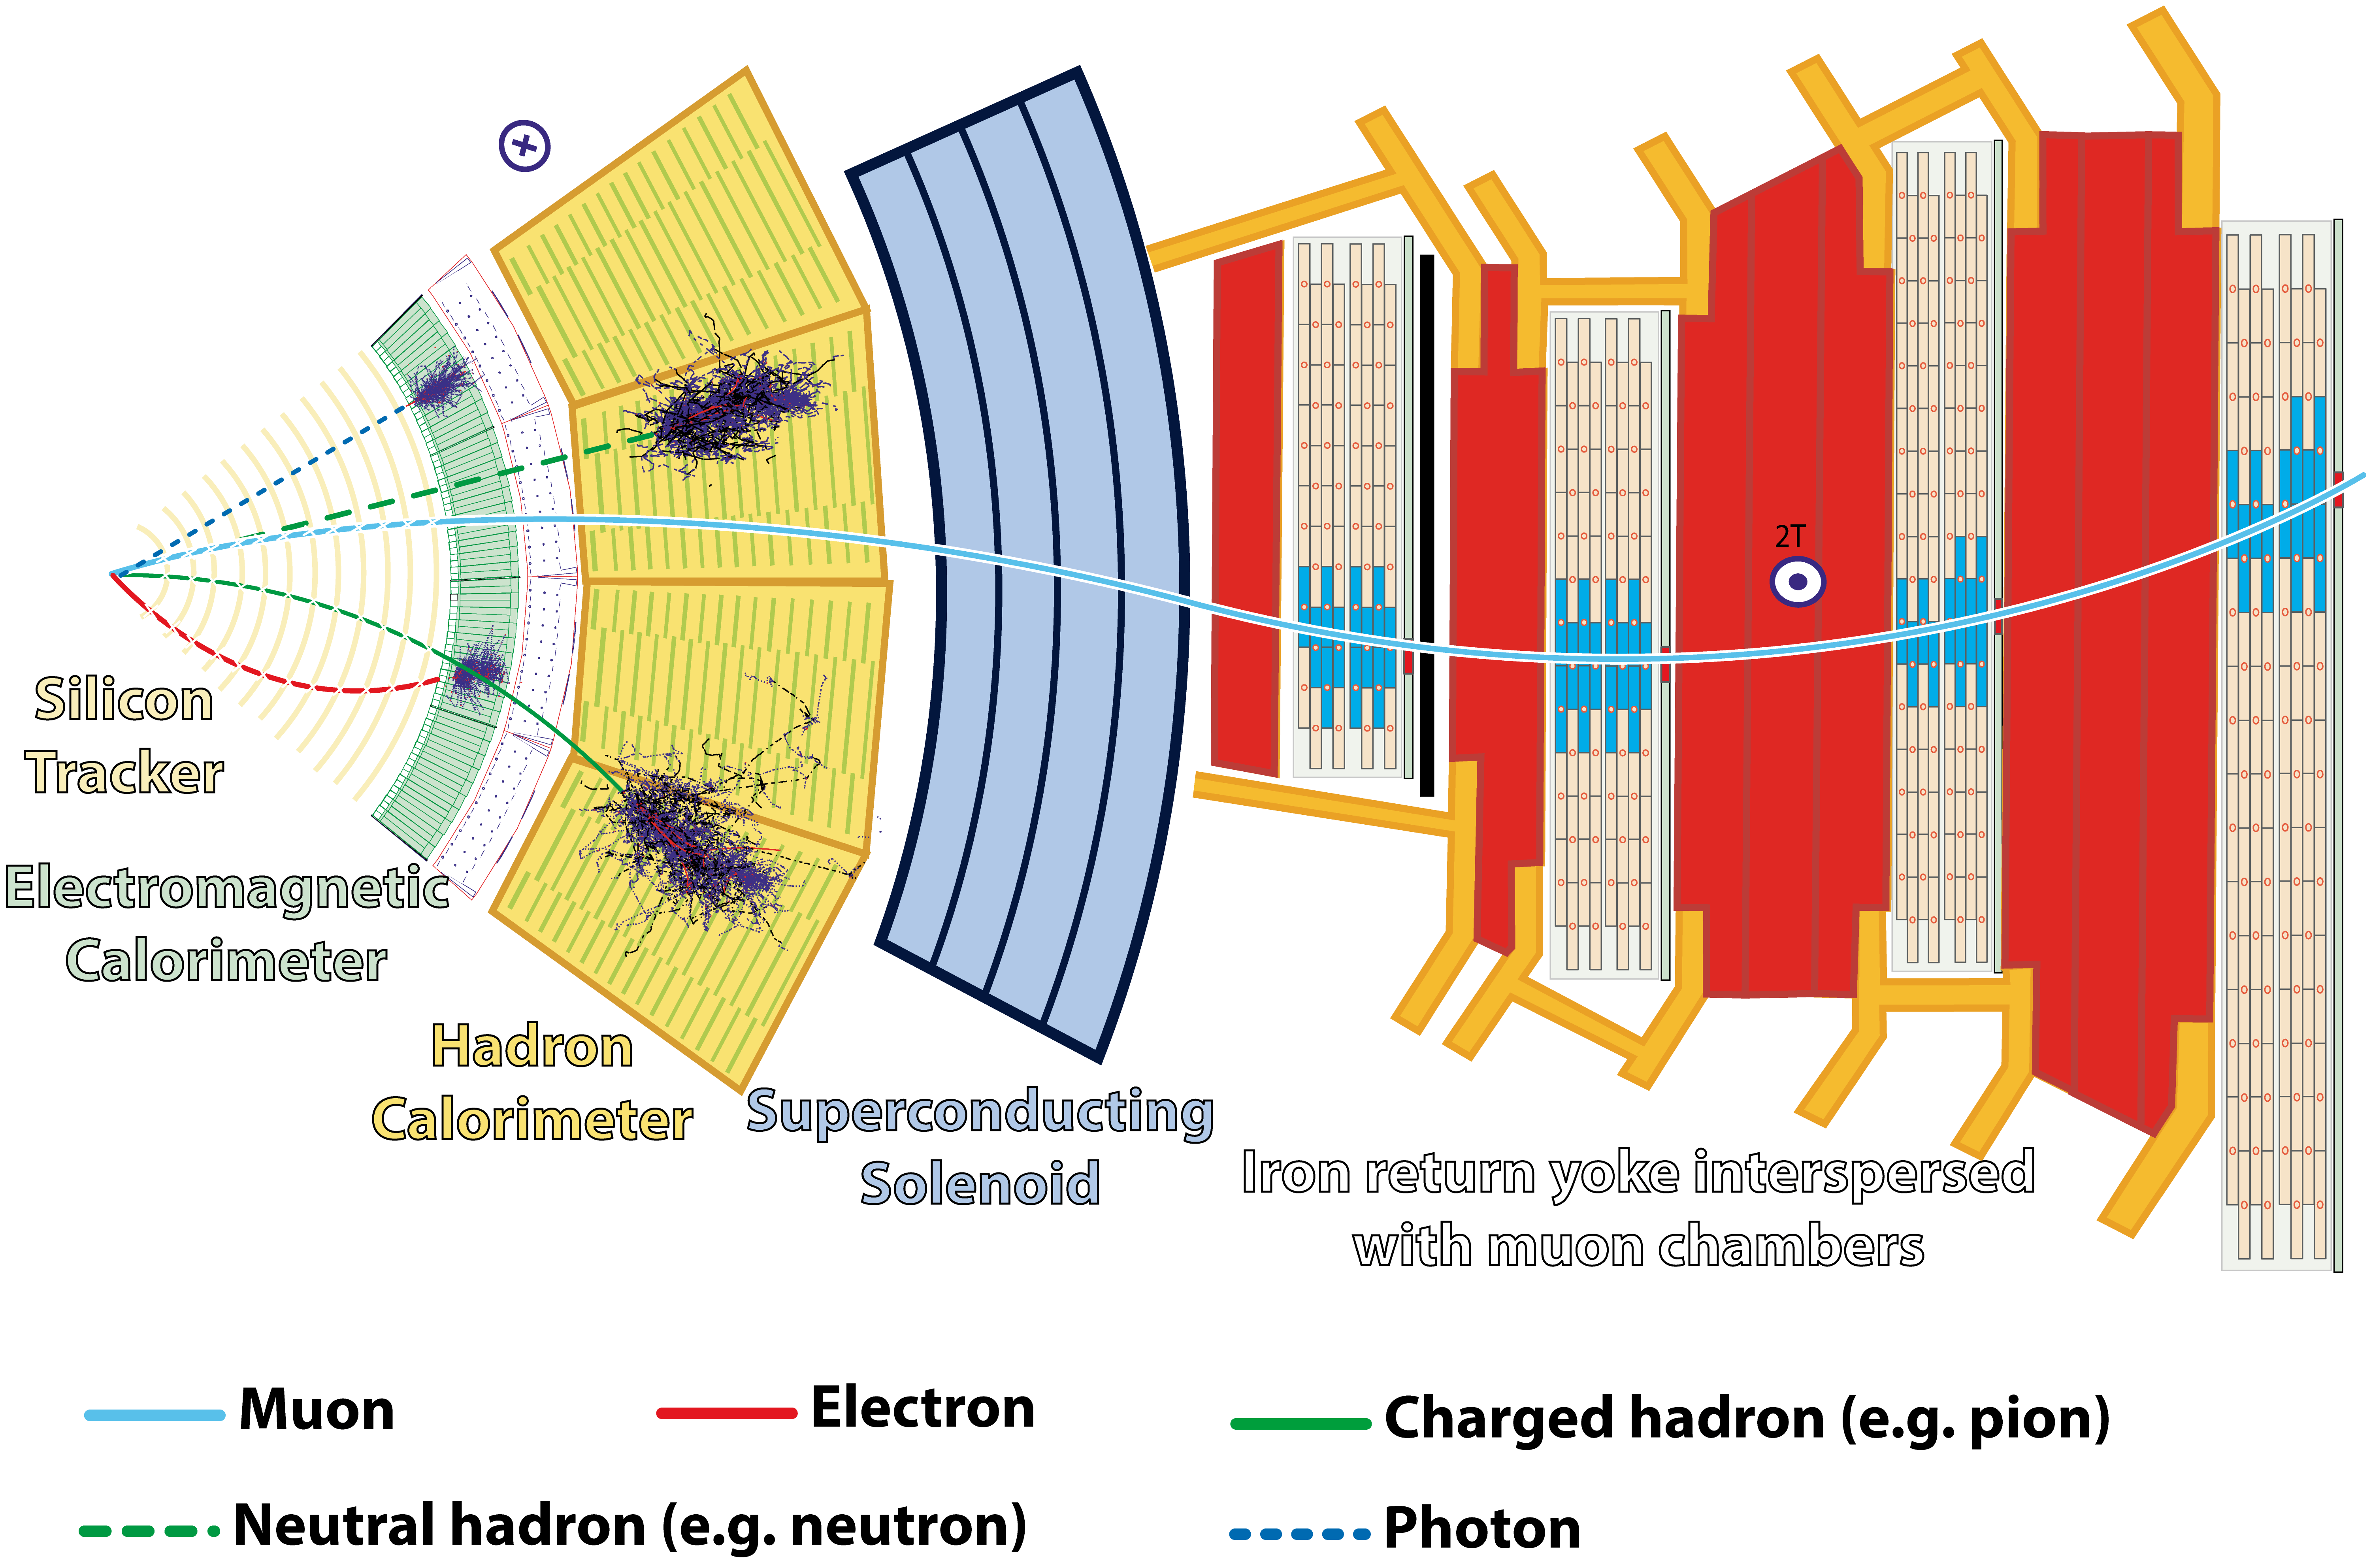
\includegraphics[width=0.85\textwidth]{pictures/CMSslice_whiteBackground.png}
\end{center}
\caption{A simplified transverse view of the CMS detector cross section \cite{CMS-PHO-GEN-2016-001}. The typical signatures of the five particle collections detected are shown.}
\label{fig:CMSslice}
\end{figure}

Within the solenoid volume there are three major subsystems:
a silicon pixel and strip tracker which measures the trajectories of charged particles,
a lead tungstate crystal electromagnetic calorimeter (ECAL) that mainly collects the energies of electrons and photons,
and a brass and scintillator hadronic calorimeter (HCAL) which stops the more penetrating hadrons.
Quartz fiber based forward calorimeters further improve hermeticity.
The measurement of muons relies on a combination of inner tracking and information from the muon chambers,
which are gas-ionization detectors embedded in the steel flux-return yoke outside the solenoid.
A detailed description of the CMS detector can be found in Reference \cite{CMS:2008}.

CMS adopts a right-handed Cartesian coordinate system, with the origin defined in the center of the detector; more precisely, the barycenter of the modules of the Tracker Outer Barrel.
The axes are oriented such that the x-axis points to the center of the LHC ring, the y-axis is orthogonal to the LHC plane pointing up, and the the z-axis lies along the anticlockwise beam direction.

\paragraph{Kinematic variables\\}
In High Energy Physics (HEP), the particle polar direction is often descrbed with its rapidity, defined as:
\begin{equation}
  \label{eq:rapidityDefinition}
  y = \frac{1}{2} ln \frac{E + p_z}{E - p_z}
\end{equation}
Difference in rapidity are invariant under Lorentz boosts along the z-axis.
In physics analyses the pseudo-rapidity is onften used in its place, since the two coincide in the ultra-relativistic limit:
\begin{equation}
  \label{eq:pseudorapidityDefinition}
  \eta = - ln \left( \tan \frac{\theta}{2} \right)
\end{equation}
where $\theta$ represents the polar angle with respect to the z-axis. The azimuthal angle, measured in the x-y plane is called $\phi$.
They are used to define a type of angular distance between two physica objects:
\begin{equation}
  \label{eq:deltaRDefinition}
  \Delta R = \sqrt{ \Delta \eta^2 + \Delta \phi^2 }
\end{equation}


\subsection{APV25 preamplifier saturation}
In late 2015 and early 2016, the CMS strip tracker encountered a signal-to-noise ratio deterioration and a loss of hit detection on tracks, particularly as instantaneous luminosity increased.
Investigation revealed that the problem stemmed from saturation in the preamplifier of the strip readout chip (APV25) under high occupancies.
Lowering the operating temperature in Run 2 unexpectedly prolonged preamplifier discharge time, resulting in charge buildup and a nonlinear response.
Muon reconstruction efficiency was also affected by preamplifier saturation.
%% The preamplifier's response was linear up to 3 MIPs, but nonlinear beyond.
This issue was resolved by adjusting the drain speed of the preamplifier \cite{Butz:2018dum} through the preamplifier feedback voltage bias (VFP), achieving a recovery of the hit efficiency to the same level as in Run 1 \cite{CMS:2021ime}.

A model for preamplifier saturation was developed and integrated into simulations, with adjustments yielding better data-model agreement.
As a consequence of these changes, for the year 2016, the detector simulations before and after the adjustment differ substantially.
The two periods, which correspond to luminosity of around 19.5 fb$^{-1}$ and 16.8 fb$^{-1}$,
are therefore analysed separately and are referred to as ``2016preVFP'' and ``2016postVFP''.
